\documentclass[a4paper]{nuist}

\begin{document}

%%%%%%%%%% 封面目录摘要 %%%%%%%%%%
% WARN: 请检查校徽是否为最新版,当前(2022 年)使用校徽为 2015 版;若不是最新版,请在 nuist_logo 文件夹中替换
% TIPS: 若标题、学院、专业名太长,可使用 \\ 进行换行,如 计算机学院 软件学院\\网络空间安全学院
% TIPS: 若不允许换行,请在 nuist.cls 文件中查找“封面”部分,并将 \parbox[b]{58mm} 中的 58 改为更大的数字
% TIPS: 2021 年论文格式要求指导老师不用加职称
\cover{南京信息工程大学本科}{生毕业论文\LaTeX 模板 }
{张三}
{************}
{某专业}
{某学院}
{路人乙}
{二O二六\hspace{0.4em} 年\hspace{0.4em} 一\hspace{0.4em} 月\hspace{0.4em} 十二\hspace{0.4em} 日}

\mytableofcontents

\maketitleofchinese{南京信息工程大学本科生毕业论文\LaTeX 模板V2022\footnote{本模板制作时间:2014年5月,最后修订于2022年1月}}{Bruce Y.P. Lee\footnote{E-mail:\url{yupenglee119@gmail.com}}、LiR\footnote{第二版修改者,E-mail:\url{stuliren@outlook.com}}、John D\footnote{2021.6版修改者,E-mail:\url{mailto:work.temp.place@outlook.com}}、B. Shen\footnote{2022版修改者,E-mail:\href{mailto:nj\_bwshen@outlook.com}{nj\_bwshen@outlook.com}}}{\LaTeX }

\abstractofchinese{这是一份南京信息工程大学本科生毕业论文\LaTeX 模板。友善提醒:本文档是非官方版,属个人兴趣产物。}{模板;南信大;毕业论文;}

\maketitleofenglish{\LaTeX\ Template for Undergraduate
    Thesis of Nanjing University of Information Science and Technology
}{Bruce Y.P. Lee、LiR、John D、B. Shen}{School of \LaTeX}

\abstractofenglish{This is a \LaTeX{~}template for the Undergraduate thesis of Nanjing University of Information Science and Technology. Caution:
    due to personal interest, not an official template.}
{template;NUIST;thesis;}

%%%%%%%%%% 封面目录摘要 %%%%%%%%%%

%%%%%%%%%% 正文 %%%%%%%%%%
% TIPS: 可以为每一章节在 body 文件夹内创建一个 .tex 文件,并以下述方式引入,也可以直接写在本文件中(不推荐)
\pagenumbering{arabic}

\section{绪言}

\subsection{\LaTeX 介绍}

\LaTeX 是一种基于\TeX 的排版系统,由美国计算机学家莱斯利·兰伯特(Leslie Lamport)在20世纪80年代初期开发,利用这种格式,即使使用者没有排版和程序设计的知识也可以充分发挥由\TeX 所提供的强大功能,能在几天,甚至几小时内生成很多具有书籍质量的印刷品。对于生成复杂表格和数学公式,这一点表现得尤为突出。因此它非常适用于生成高印刷质量的科技和数学类文档。这个系统同样适用于生成从简单的信件到完整书籍的所有其他种类的文档\footnote{摘自百度百科}。如果想有更多的了解,可以看看比较经典的入门教程。

\subsection{本模板介绍}

鉴于Microsoft Word 编写论文排版工作量大且枯燥,为了实现论文的排版的自动化、规范化,按照《南京信息工程大学本科生毕业论文(设计)撰写排版规范》编写了可用于南京信息工程大学本科生毕业论文的\LaTeX 模板。
\section{NUIST模板介绍}

\subsection{适合人群}

所有对\LaTeX 感兴趣的南京信息工程大学本科毕业生。

由于使用者可能有一些个人化的需求,本模板可能要求使用者愿意通过搜索引擎等方式解决该问题。

\subsection{使用环境}

由于现在 LuaLaTeX 排版引擎已经比较成熟,所以这里采用 LuaLaTeX 和 \CTeX{} 宏集解决中英文混排问题。

本模板的推荐使用环境为:

\begin{enumerate}[1、]
    \item Windows 10
    \item TeX Live 最新发行版全量安装(2020和2021可以正常编译)
    \item Visual Studio Code 和 Visual Studio Code LaTeX Workshop Extension(作者为 James Yu)
\end{enumerate}

\subsection{字体}

模板使用宋体、黑体、Times New Roman和楷体。根据2021.6版修订者的经历,建议使用Windows系统下的中易字库(SimSun、SimHei、SimKai)和Times New Roman。笔者一开始使用的是思源宋体(Source Han Serif),但论文打印稿被答辩老师一眼看出使用的不是常见的宋体……

使用 AutoFakeBold 和 AutoFakeSlant 作为粗体和斜体。

因此,笔者建议 Linux 用户和 Mac OS 用户请自行安装中易字库(Times New Roman 倒是很容易安装,Arch Linux下直接有包 \url{https://aur.archlinux.org/packages/ttf-ms-fonts/}),相信这对各位来说不是什么难事。

\subsection{文档类的选取}

模版的文档类是基于\CTeX{} 宏集中自带的ctexart文档类来实现的\cite{x5},还用到了一些常用的宏包,编译时要保证自己的系统中已经安装好了这些宏包,如果用户使用的是全量安装的 TeX Live就没有问题。

\subsection{参考文献编译方式}

模板推荐使用\verb|\bibliography{}|命令处理参考文献,借助“GB/T 7714—2015 BibTeX Style”\cite{x6},模板使用者可以放心大胆地将参考文献的排版工作交给\LaTeX ,而无需手动调整每条参考文献的格式,详见\ref{sec:ref}

\section{模板中命令的使用方法}

\subsection{分级标题}

模板各级标题的命令如表~\ref{table_title_command}~所示:

\begin{table}[htbp!]
    \centering
    \caption{分级标题命令}
    \label{table_title_command}
    \begin{tabular}{ccccc}
        \toprule
        命令 & \verb|\section| & \verb|\subsection| & \verb|\subsubsection| & \verb|\paragraph| \\
        \midrule
        作用 & 一级标题        & 二级标题           & 三级标题              & 四级标题          \\
        \bottomrule
    \end{tabular}
\end{table}

虽然学校排版规范最低允许四级标题,但是ctexart文档类的自动编号应该只支持到三级标题,因此四级标题需要自行编号。

\subsection{NUIST模板中新定义命令介绍}

这里一一介绍下NUIST本科论文模板中的新定义的命令:

{
\color{blue}
\begin{enumerate}
    \item \verb|\cover|,用于生成论文封面内容和声明页;
    \item \verb|\mytableofcontents|,用于生成目录页内容;
    \item \verb|\maketitleofchinese|,用于生成中文标题、姓名及单位信息
    \item \verb|\maketitleofenglish|,用于生成英文文标题、姓名及单位信息
    \item \verb|\abstractofchinses|,用于生成中文摘要;
    \item \verb|\abstractofenglish|,用于生成英文摘要;
    \item \verb|\thanking|,用于生成致谢部分的标题;
\end{enumerate}
}

\subsection{命令用法详解}

\LaTeX/\TeX 中的命令都是以$\backslash$(反斜杠)开始的。命令又分为两种,一种是无参数命令,起声明和执行特定任务作用;另一种 是有参数命令。带参命令的参数又有两种类型一种是可选参数(用[ ]来框住,可省略该项参数),另一种是必选参数(用\{ \}来框住)。

本模板中自定义的命令有只有一个是不带参的命令,即\verb|\mytableofcontents|,其余都是带参命令。

\subsubsection{带参命令用法}

\verb|\cover|\{val1\}\{val2\}\{val3\}\{val4\}\{val5\}\{val6\}\{val7\}这里val1-val6分别表示填入的信息依次为:val1 =论文题目,val2 =姓名,val3 =学号,val4 =学院,val5 =专业,val6 =导师,val7 =年月日。例如如下代码,就生成了本说明文档的封面。

{
\color{green!50!black}
\begin{lstlisting}[breaklines=true,]
\cover{南京信息工程大学本科生毕业论文\LaTeX 模板 \\Version $2022$}
{路人甲}
{20170000888}
{\LaTeX 学院}
{某专业}
{路人乙}
{二O二一\hspace{0.4em} 年\hspace{0.4em} 六\hspace{0.4em} 月\hspace{0.4em} 五\hspace{0.4em} 日}
\end{lstlisting}
}

那接下来看看剩下的几个命令的参数数量及参数所对应的内容是什么:

{
\color{blue}
\begin{itemize}
    \item \verb|\mytableofcontents|,无参数命令
    \item \verb|\maketitleofchinese|\{论文标题\}\{姓名\}\{学院\}
    \item \verb|\maketitleofenglish|\{英文标题\}\{英文姓名或拼音\}\{学院\}
    \item \verb|\abstractofchinses|\{中文摘要内容\}\{中文关键词\}
    \item \verb|\abstractofenglish|\{英文摘要内容\}\{中文关键词\}
    \item \verb|\thanking|\{致谢内容\}
\end{itemize}
}

下面再来举个例子,如下面的这些命令,就可以分别产生本文档前面的中文标题、摘要和英文标题、摘要。

{
\color{green!50!black}
\begin{lstlisting}[breaklines=true,]
\maketitleofchinese{南京信息工程大学本科生毕业论文\LaTeX 模板V2021.6\footnote{本模板制作时间:2014年5月,修订于2022年1月}}{路人甲}{\LaTeX}

\abstractofchinese{这是一份南京信息工程大学本科生毕业论文\LaTeX 模板。友善提醒:本文档是非官方版,属个人兴趣产物。}{模板;南信大;毕业论文;}
    
\maketitleofenglish{\LaTeX\ Template for Undergraduate Thesis of Nanjing University of Information Science and Technology}{Some Guy}{School of \LaTeX}
    
\abstractofenglish{This is a \LaTeX{~}template for the Undergraduate thesis of Nanjing University of Information Science and Technology. Caution: due to personal interest, not an official template.}{template;NUIST;thesis;}
\end{lstlisting}
}

\subsubsection{不带参命令用法}

不带参命令\verb|\mytableofcontents| 用来生成目录。只需原封不动的打出相应命令,编译就会自动执行相应的排版操作,如用\verb|\mytableofcontents|就可以在命令的位置生成目录页。

\section{排版数学公式}

\LaTeX 强大之处就在于其有很强的数学公式排版能力,如果再加上amsmath宏包,更是如虎添翼。其中\$  \$表示行内公式,如\verb|$a^2+b^2=c^2$|会生成$a^2+b^2=c^2$,而\$\$  \$\$表示行间公式,其实这还不算什么,最重要的是即使处理高度比较高的行间公式时,\LaTeX 也会自动处理而不会使文章中的行距突兀地增大,如$x_{1,2}= \frac{-b\pm \sqrt{b^2-4ac}}{2a}$,而命令\verb|$$a^2+b^2=c^2$$|,会产生$$a^2+b^2=c^2$$
上面的就是一个行间公式。

\begin{equation}\label{fomula}
    \begin{cases}
        \dfrac{du}{dt}=-\dfrac{\partial \phi}{\partial x}+fv \\[1.5ex]
        \dfrac{dv}{dt}=-\dfrac{\partial \phi}{\partial y}-fu \\[1.5ex]
        \dfrac{\partial \phi}{\partial p}=-\dfrac{1}{\rho}   \\[1.5ex]
        p= \rho RT                                           \\[1.5ex]
        \dfrac{\partial u}{\partial x}+\dfrac{\partial v}{\partial y}+
        \dfrac{\partial \omega}{\partial p}=0                \\[1.5ex]
        \dfrac{\partial T}{\partial t}+\overrightarrow{V}\times \nabla_pT-(\Gamma_d-\Gamma)\omega=\dfrac{Q}{c_p}
    \end{cases}
    \text{。}
\end{equation}

式~\ref{fomula}~中为气象上常用的大气运动基本方程组,而且这是一个带编号的公式。

其他公式示例

多行公式使用\&对齐
\begin{equation}
    \begin{aligned}
        A   & =1   \\
        BBB & =222
    \end{aligned}
\end{equation}

无序号公式 equation*
\begin{equation*}
    x=1
\end{equation*}

公式排版就简单介绍到这里吧,因为对笔者所学的专业来说,论文中很少涉及这方面内容,当然个别研究领域可能会出现许多公式,那就是比较高深的领域了,一般是做动力机理或数值模拟研究时常会用到公式,如果有兴趣可以参见\cite{x1}。

\section{排版图片}

\subsection{支持图片格式}

模板支持的图片格式有:jpg,pdf,eps,png等。既然选择了 \LaTeX,那就尽量使用pdf,eps等矢量图。

\subsection{插入图片方法}

论文中图是很重要的,俗语曰:“一图胜千言,有图有真相”,总之,有图,言者能言之凿凿,观者能察之切切。

\begin{figure}[htbp]
    \centering
    
\includegraphics[width=0.6\textwidth]{figs/color/face.png}
    \caption{南京信息工程大学本科生毕业论文\LaTeX 模板封面展示}
    \label{nuist_face}
\end{figure}

图\ref{nuist_face}就是插入到文档中的图片。

\subsection{并列图及添加子图标题}

大家在做论文时的时候经常需要两幅图并排的情况,下面来看看\LaTeX 是怎样精确控制并排图片占位大小的,从而使其各占一半水平空间。如图\ref{cn_map}:

\begin{figure}[htbp!]
    \centering
    \includegraphics[width=0.5\textwidth]{figs/color/china1.png}\includegraphics[width=0.5\textwidth]{figs/color/china2.png}
    \caption{中国地图展示(左图为素颜,右图为彩妆)}
    \label{cn_map}
\end{figure}

是不是感觉图\ref{cn_map}的标题不太专业,也想给左右两个子图各加一个标题?那其实也很简单,模板引入了subfigure宏包实现。实现后效果如图\ref{subfig_cn_map}:

\begin{figure}[htbp!]
    \centering
    \subfigure[素颜\label{fig:sub1}]{\includegraphics[width=0.5\textwidth]{china1.png}}\subfigure[彩妆\label{fig:sub2}]{\includegraphics[width=0.5\textwidth]{china2.png}}
    \caption{中国地图展示}
    \label{subfig_cn_map}
\end{figure}

当然我们在引用的时候,可以引用母图,如图\ref{subfig_cn_map},也可以引用子图,如图\ref{subfig_cn_map}\subref{fig:sub1},图\ref{subfig_cn_map}\subref{fig:sub2}。

好了让我们来看实现的代码吧:

{
\color{green!50!black}
\begin{lstlisting}[breaklines=true,]
\begin{figure}[htbp!]
    \centering
    \subfigure[素颜\label{fig:sub1}]{\includegraphics[width=0.5\textwidth]{china1.png}}\subfigure[彩妆\label{fig:sub2}]{\includegraphics[width=0.5\textwidth]{china2.png}}
    \caption{中国地图展示}
    \label{subfig_cn_map}
\end{figure}
\end{lstlisting}
}

最后再给出一个例子,例如大家在做EOF分析时,可能要两个模态之间进行对比,我们知道每一个模态场都有一个时间序列与其对应,所以这样我们还可能用到$2\times 2$形式的图片排列方式,如图\ref{fig:eof_12}。

\begin{figure}[htbp]
    \center
    \subfigure[第一模态]{\label{eof_1}
        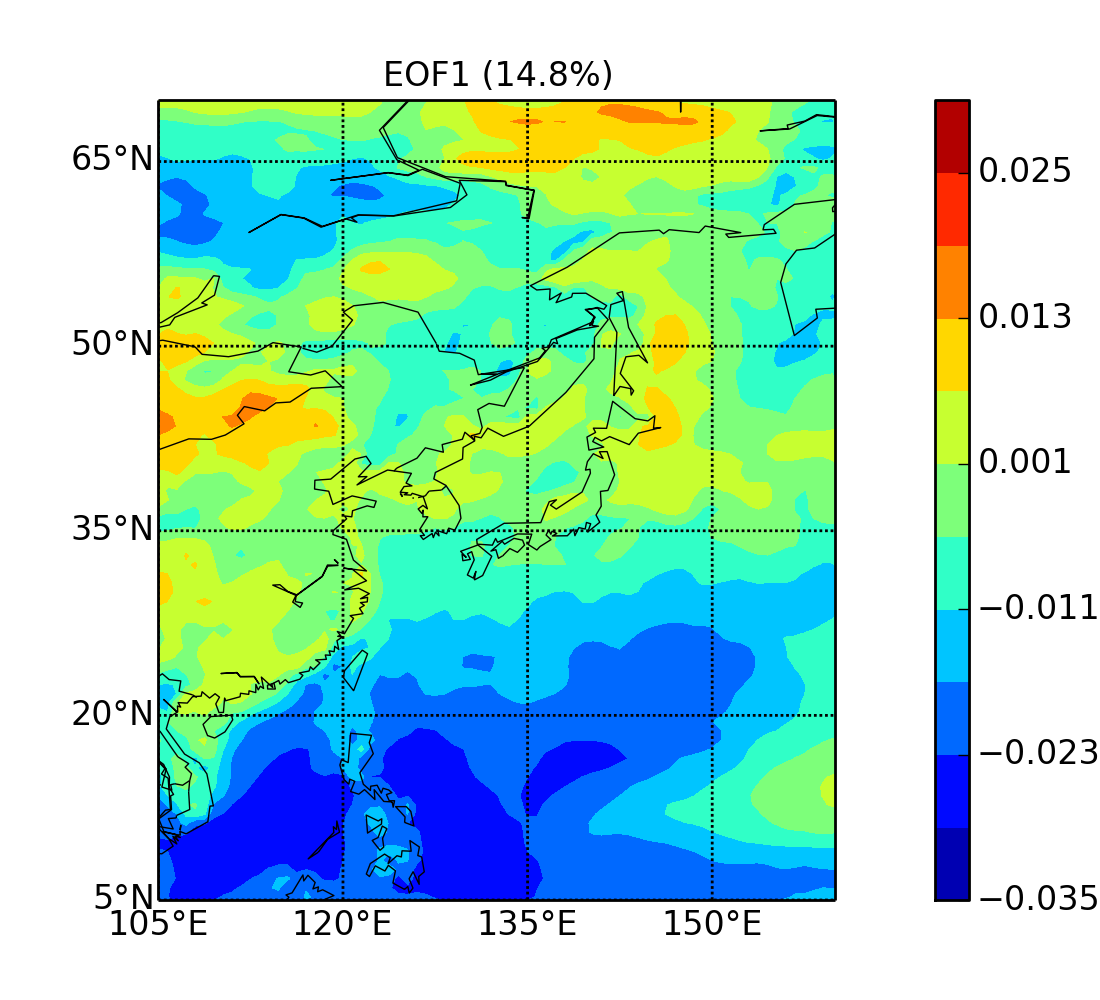
\includegraphics[width=0.4\textwidth]{eof1.png}
    }\subfigure[第二模态]{\label{eof_2}
        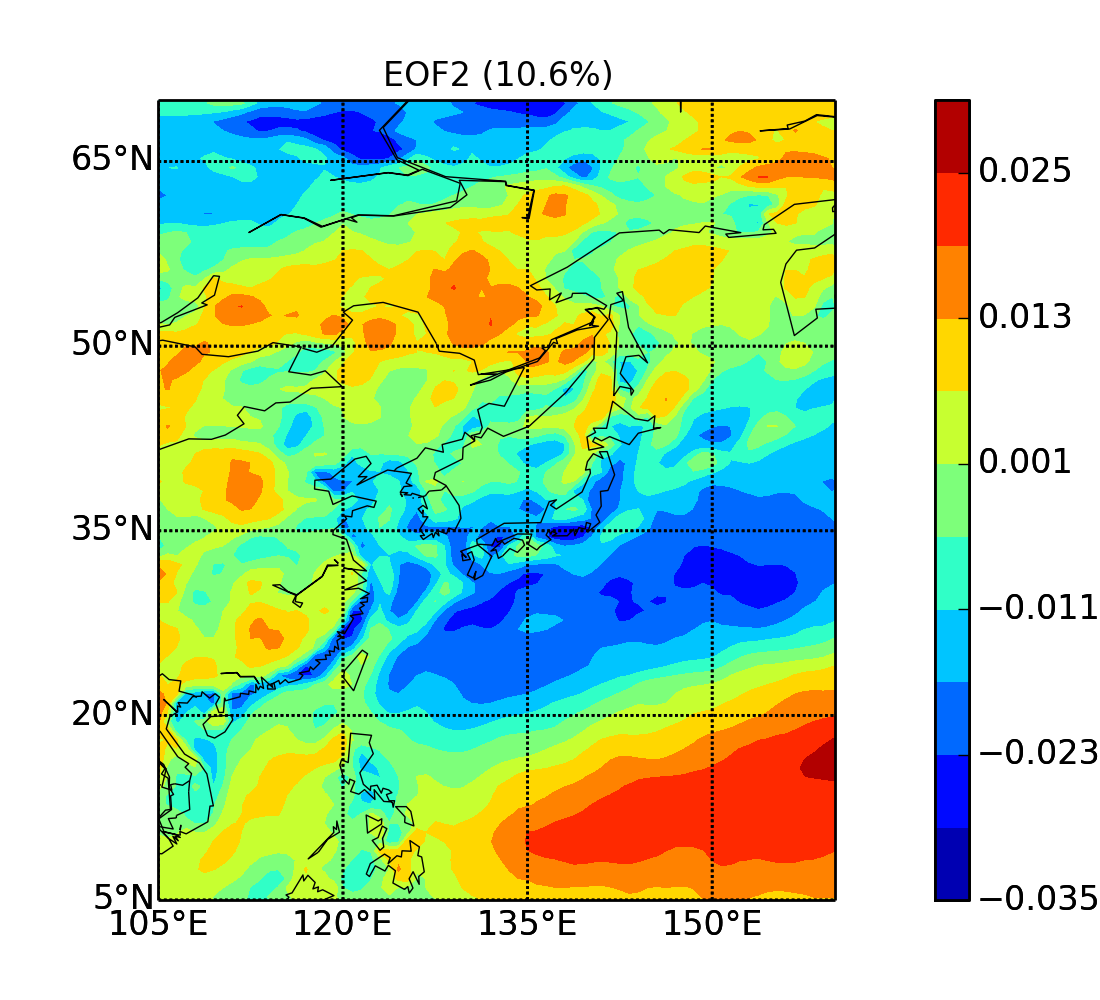
\includegraphics[width=0.4\textwidth]{eof2.png}
    }
    \\
    \subfigure[第一模态对应的时间系数]{\label{eof_t1}
        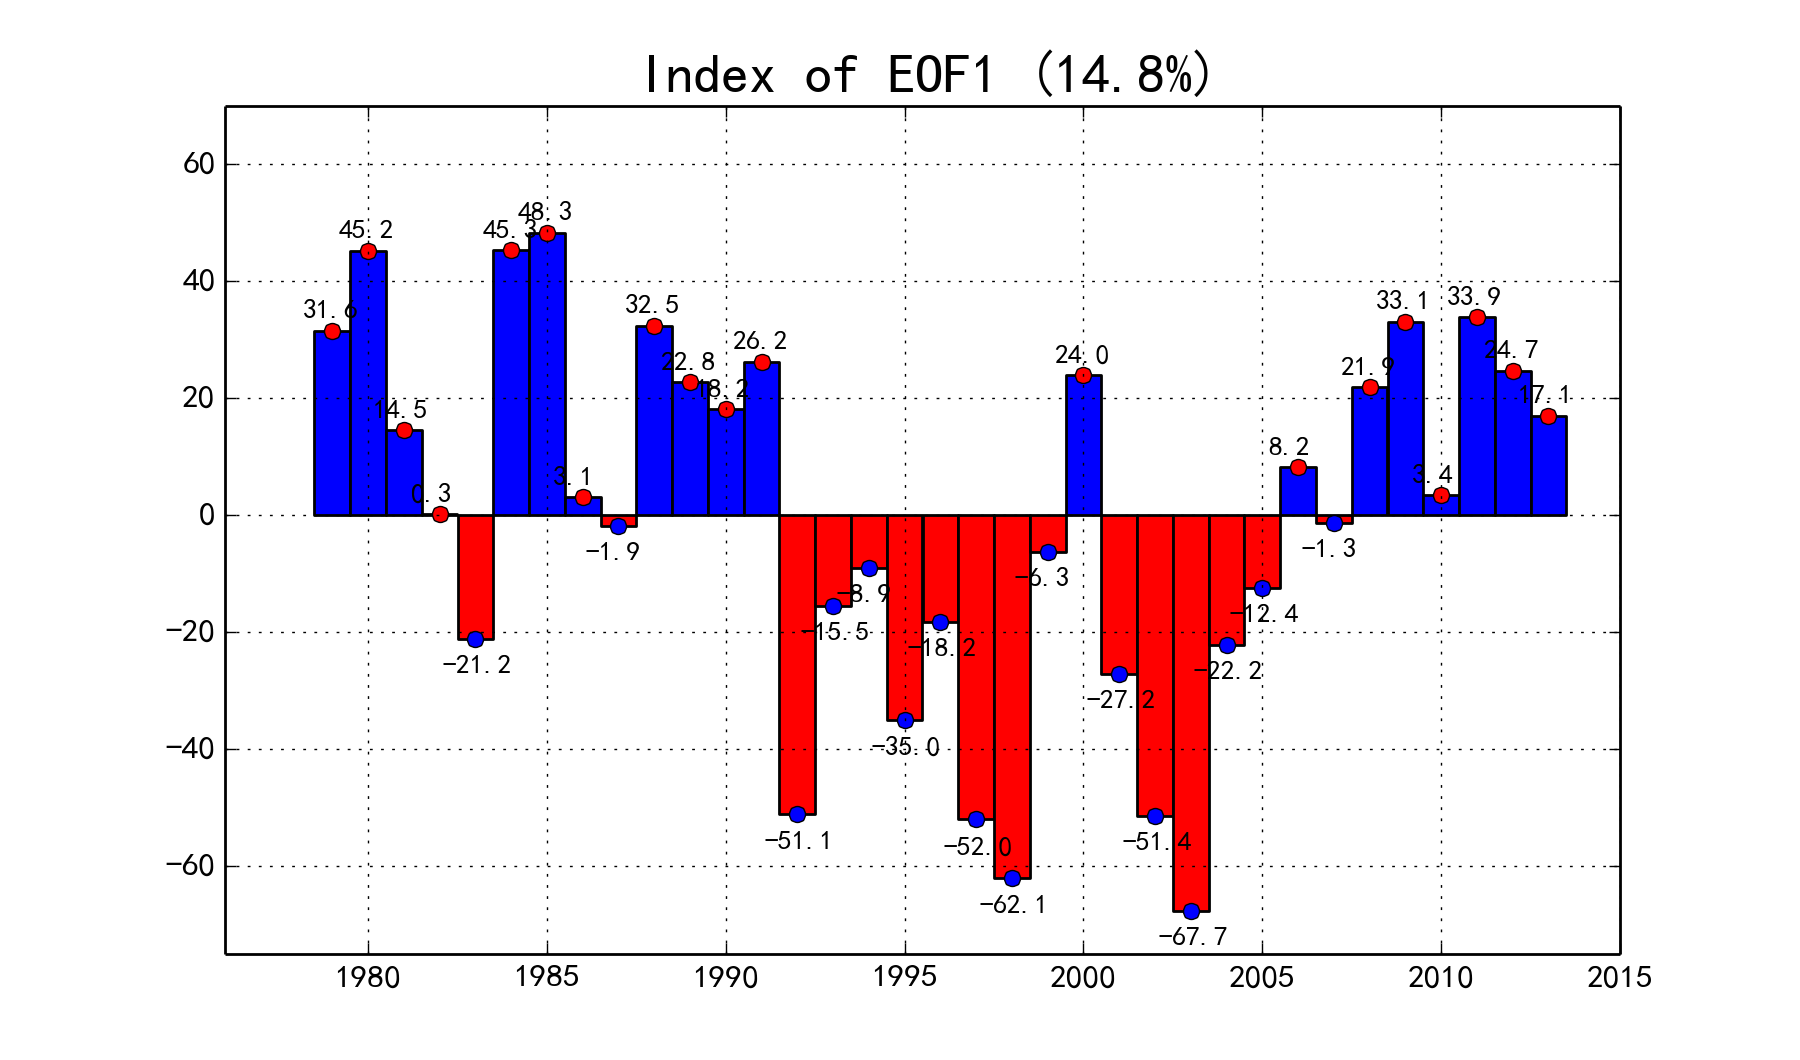
\includegraphics[width=0.4\textwidth]{t1.png}
    }\subfigure[第二模态对应的时间系数]{\label{eof_t2}
        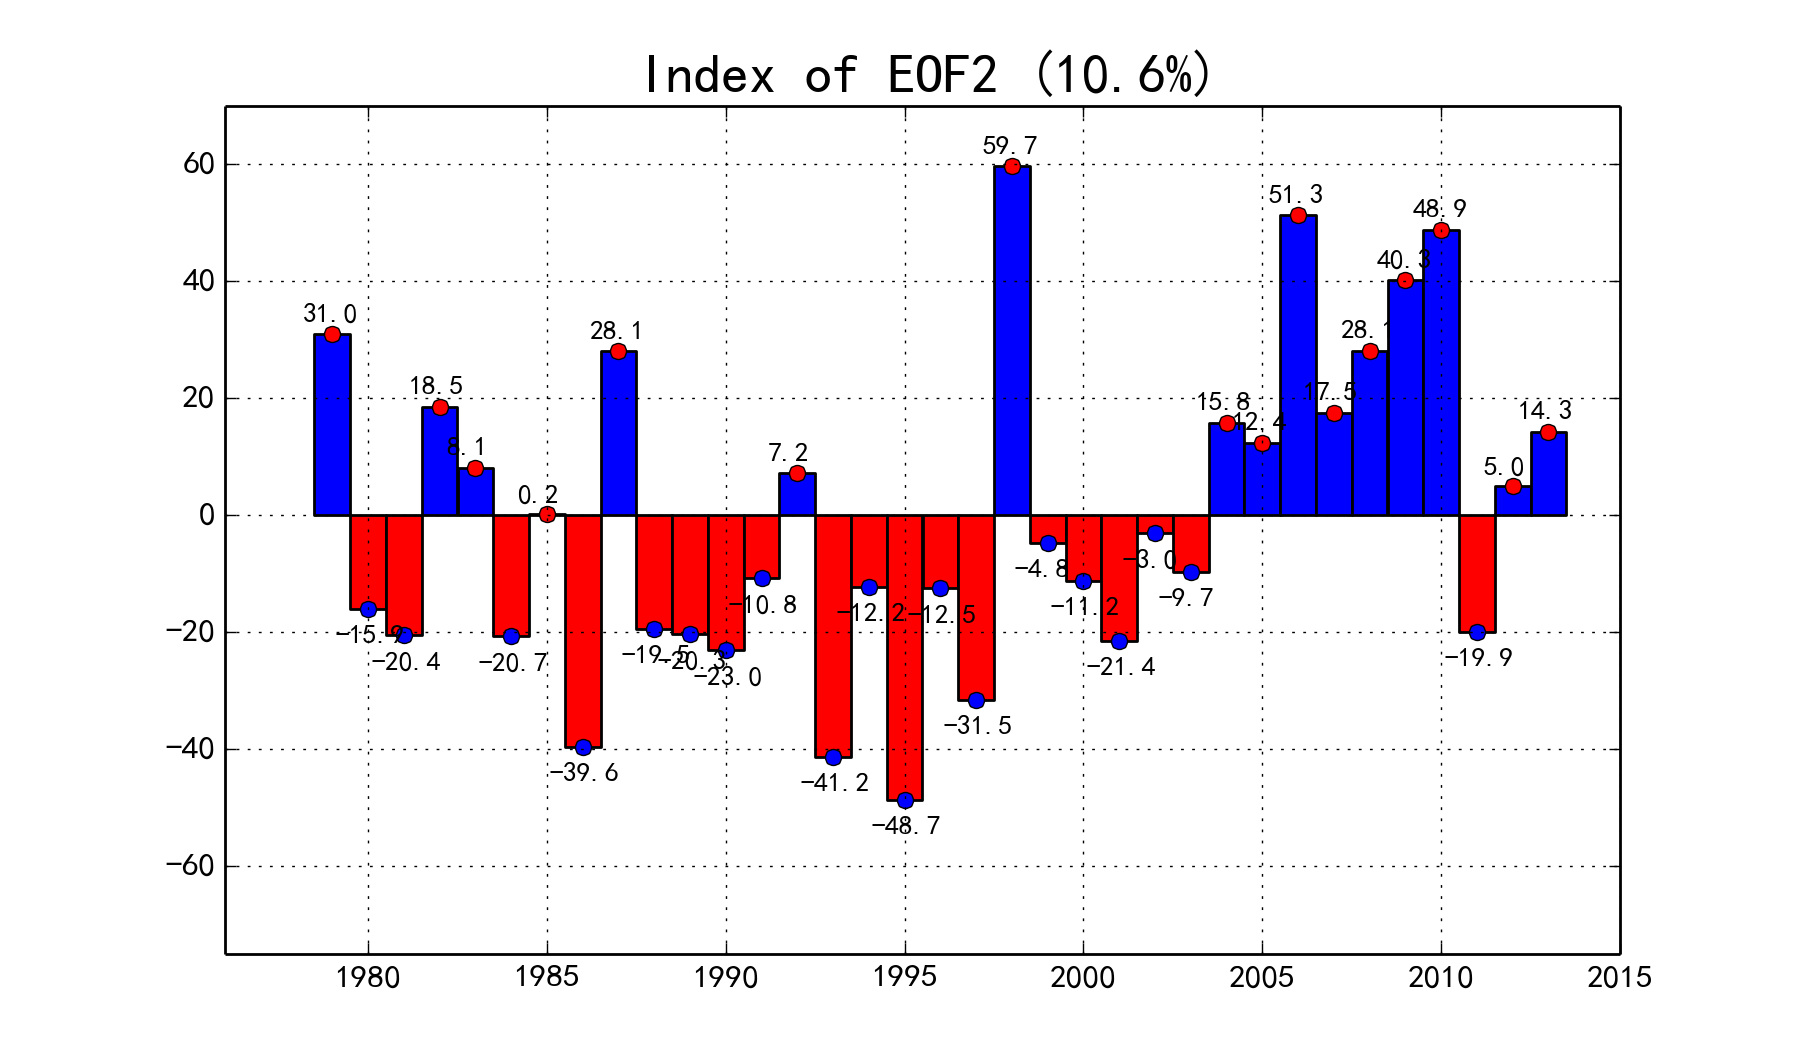
\includegraphics[width=0.4\textwidth]{t2.png}
    }
    \caption{ABLH的EOF分析结果(第一第二模态及其时间系数)}\label{fig:eof_12}
\end{figure}

我们可以用下面的命令来实现:

{
\color{green!50!black}
\begin{lstlisting}[breaklines=true,]
\begin{figure}[htbp]
    \center
    \subfigure[第一模态]{\label{eof_1}
        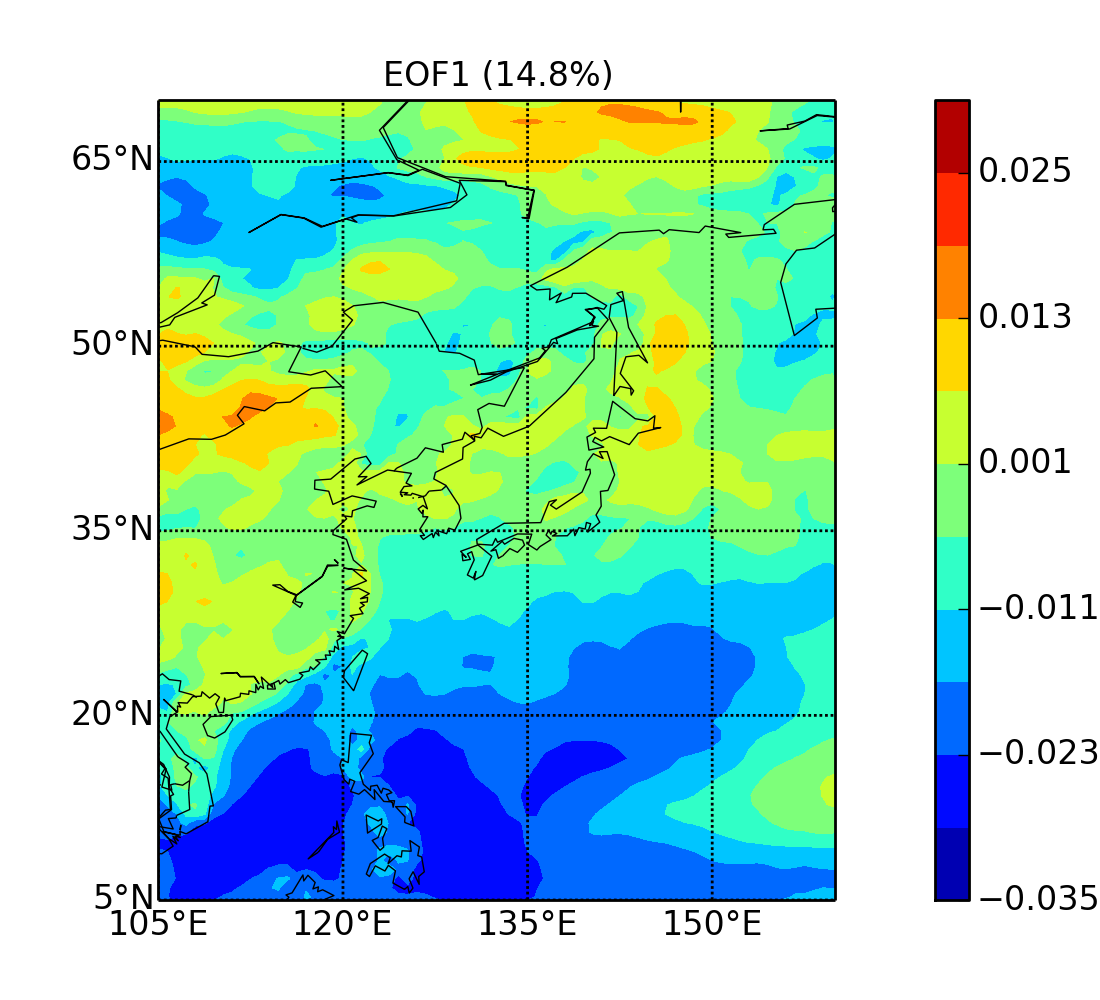
\includegraphics[width=0.4\textwidth]{eof1.png}
    }\subfigure[第二模态]{\label{eof_2}
        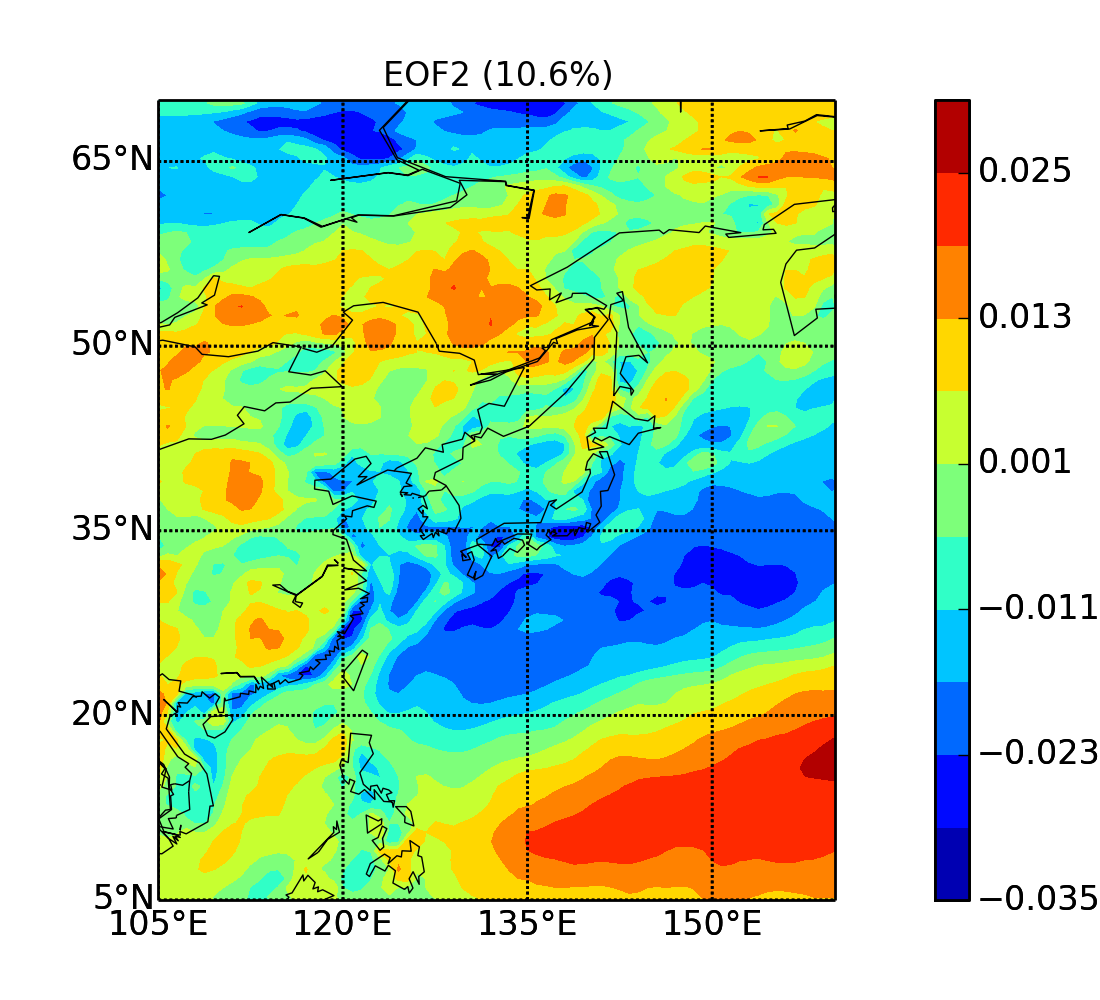
\includegraphics[width=0.4\textwidth]{eof2.png}
    }
    \\
    \subfigure[第一模态对应的时间系数]{\label{eof_t1}
        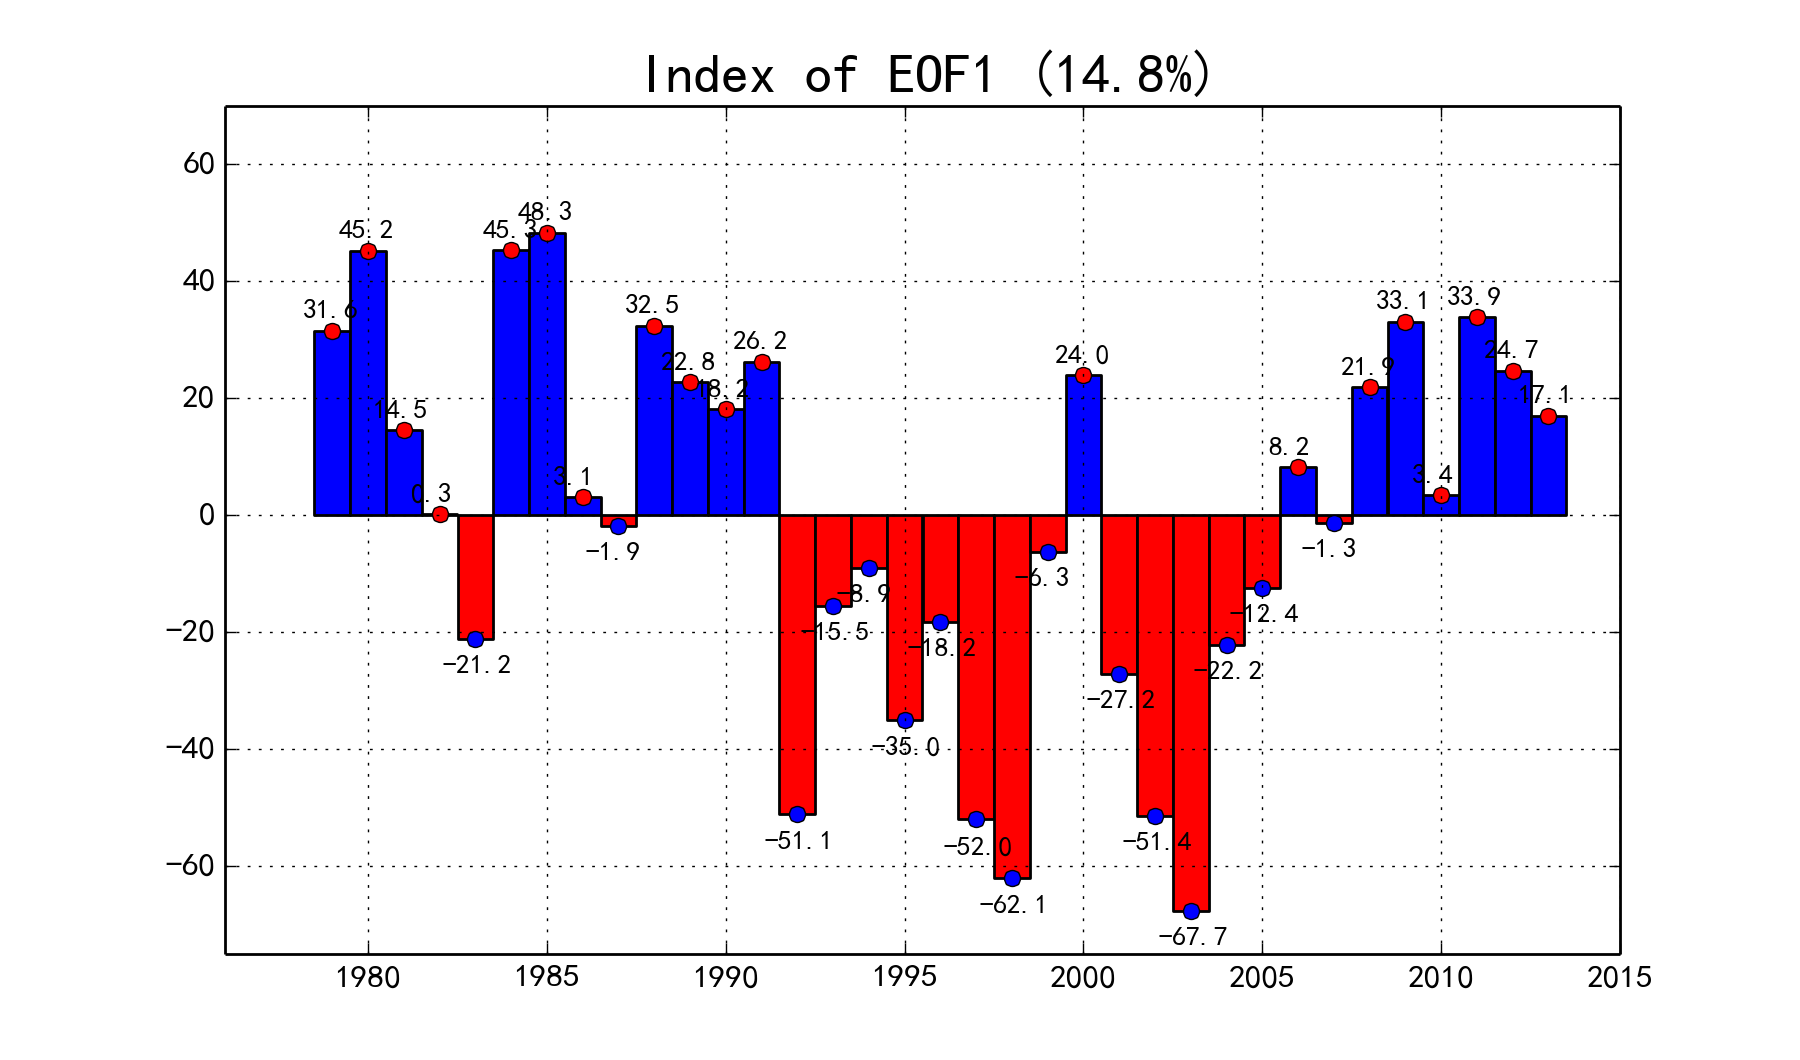
\includegraphics[width=0.4\textwidth]{t1.png}
    }\subfigure[第二模态对应的时间系数]{\label{eof_t2}
        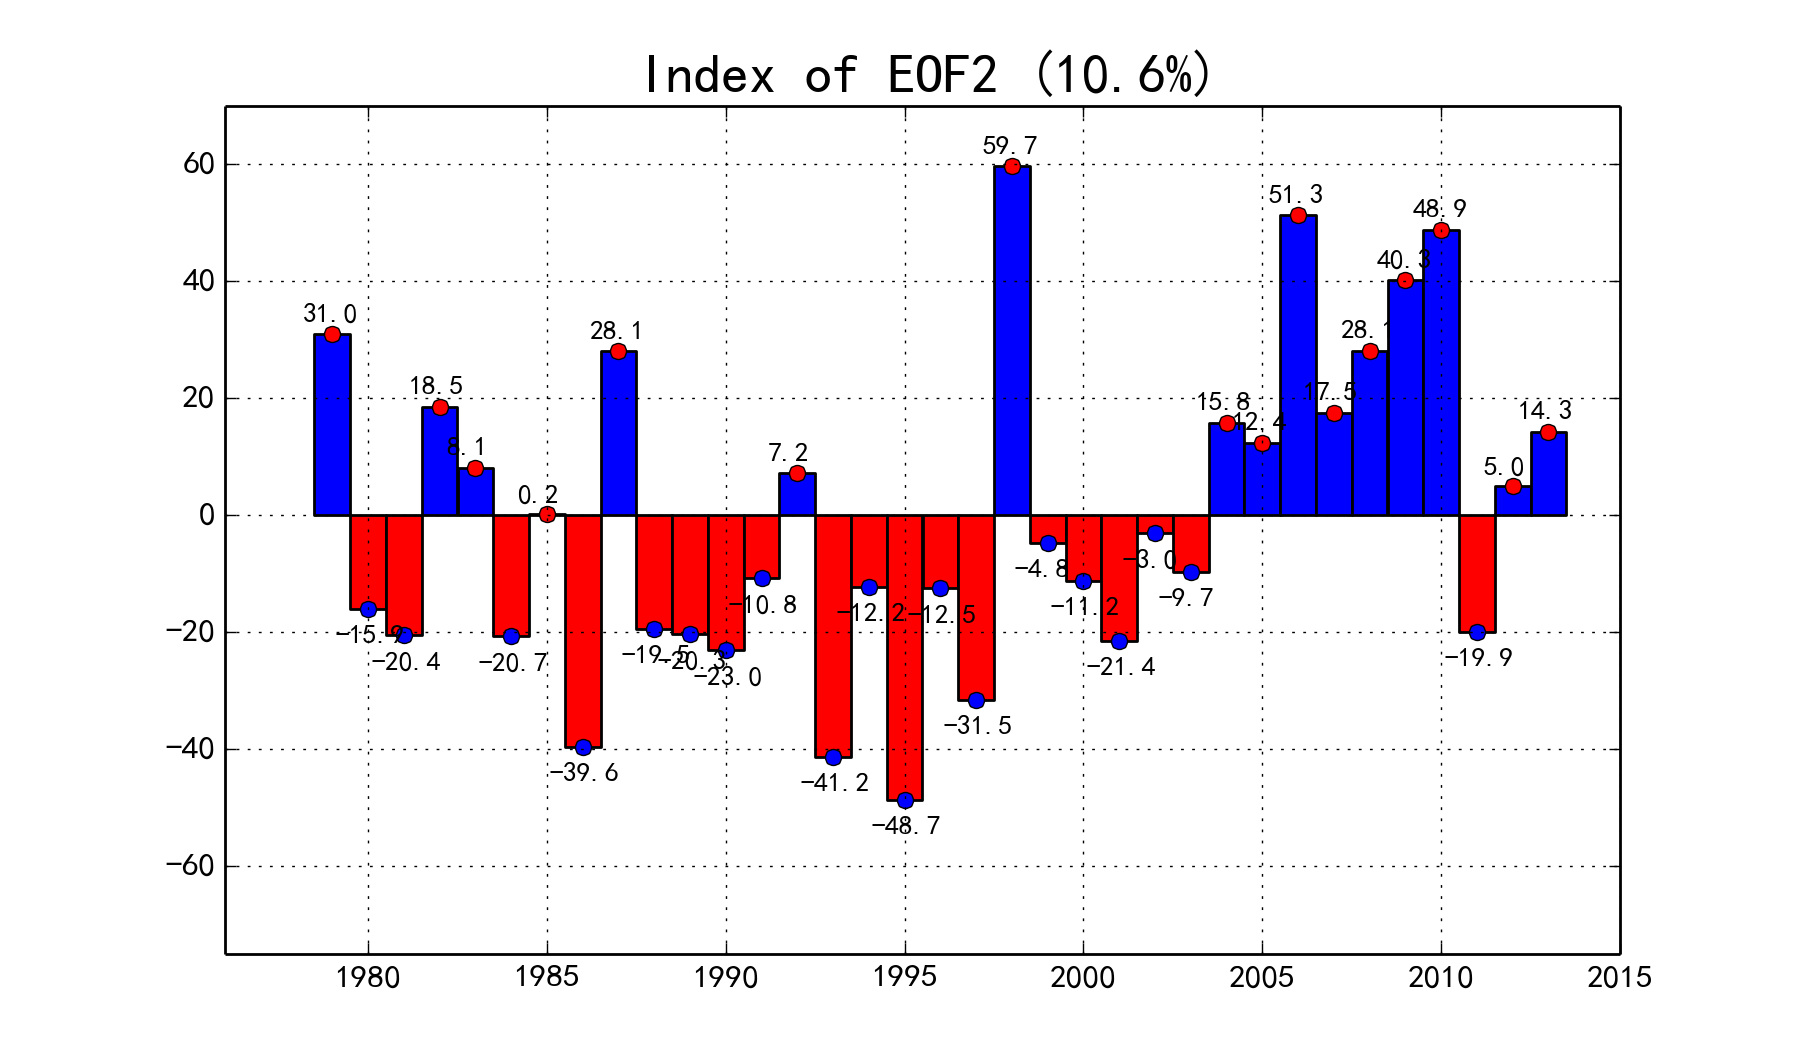
\includegraphics[width=0.4\textwidth]{t2.png}
    }
    \caption{ABLH的EOF分析结果(第一第二模态及其时间系数)}\label{fig:eof_12}
\end{figure}
\end{lstlisting}
}

朋友们应该也发现奥秘所在了,对,就是那个双斜线 $\backslash\backslash$ 的作用,双斜线在\LaTeX 排版系统中就是换行的命令,知道了这一点,大家可以随意安排自己的图片了,可以用$2\times 3$或者$3\times 2$来摆放自己插图了。

\subsection{图片文件夹的指定}

细心的朋友可能会发现生成\ref{subfig_cn_map}和图\ref{cn_map}所用的代码在指定图片路径时的写法不同,一种是相对路径,另一种是只有图片名称。这是为什么呢?原因很简单。为了在写作时引用图片方便,本文在导言区写上这样的\verb|\graphicspath{{figs/color/}}|一名命令,来宏观地指定图片所存放的位置。

这一功能的好处就是,对于有的同学电子文档和打印文档所用图片色彩格式不同,这样只要一条命令就可以切换到另一个文件夹了,比较实用。

\section{排版表格}

\LaTeX 中生成简单的表格还是比较方便的,可以用tabular 环境来实现。模板引入了 booktabs 包实现三线表样式,下面就来做一个论文中经常用到的三线表,如表~\ref{table_1}~。

\begin{table}[htbp!]
    \centering
    \caption{本模板中部分使用的宏包及功能}
    \label{table_1}
    \begin{tabular}{ccccccccc}
        \toprule
        宏包名称 & amsmath  & caption  & geometry & ulem   & xcolor & setspace & hyperref \\
        \midrule
        作用     & 数学公式 & 定制标题 & 页面设置 & 下划线 & 颜色   & 行距     & 超链接   \\
        -        & -        & -        & -        & -      & -      & -        & -        \\
        \bottomrule
    \end{tabular}
\end{table}

如果表格比较长,那就要用到跨页表格排版宏包longtable了(模板中已引入该宏包)。基本的表格排版情况就介绍这么多,大家感兴趣自己慢慢去探索吧。

对于复杂表格,可以使用在线工具 Tables Generator \url{https://www.tablesgenerator.com/}

\section{排版代码}

\subsection{排版算法伪代码}

本模板引入了 algorithm 和 algorithmic 包排版伪代码,伪代码排版包有较多版本,具体可以参考 \url{https://tex.stackexchange.com/questions/229355/algorithm-algorithmic-algorithmicx-algorithm2e-algpseudocode-confused#answer-230789}

伪代码排版示例

\begin{algorithm}[htbp]
    \floatname{algorithm}{算法}                         % 将 Algorithm 替换为 算法
    \renewcommand{\algorithmicrequire}{\textbf{输入:}} % 将 Require   替换为 输入
    \renewcommand{\algorithmicensure}{\textbf{输出:}}  % 将 Ensure    替换为 输出
    \caption{算法名}
    \label{alg:algorithm1}
    \begin{algorithmic}[1] % [1] 使用行号
      \REQUIRE 输入
      \ENSURE 输出

      \STATE 某种操作

      \WHILE{while 循环控制}
        \STATE 某种操作
      \ENDWHILE

      \FOR{for 循环控制}
        \STATE 某种操作
      \ENDFOR

      \IF{if 条件控制}
        \STATE 某种操作
      \ELSE
        \STATE 某种操作
      \ENDIF

      \STATE \textbf{return} 返回值
    \end{algorithmic}
\end{algorithm}

代码

\begin{lstlisting}[breaklines=true,]
\begin{algorithm}[htbp]
    \floatname{algorithm}{算法}                         % 将 Algorithm 替换为 算法
    \renewcommand{\algorithmicrequire}{\textbf{输入:}} % 将 Require   替换为 输入
    \renewcommand{\algorithmicensure}{\textbf{输出:}}  % 将 Ensure    替换为 输出
    \caption{算法名}
    \label{alg:algorithm}
    \begin{algorithmic}[1] % [1] 使用行号
      \REQUIRE 输入
      \ENSURE 输出

      \STATE 某种操作

      \WHILE{while 循环控制}
        \STATE 某种操作
      \ENDWHILE

      \FOR{for 循环控制}
        \STATE 某种操作
      \ENDFOR

      \IF{if 条件控制}
        \STATE 某种操作
      \ELSE
        \STATE 某种操作
      \ENDIF

      \STATE \textbf{return} 返回值
    \end{algorithmic}
\end{algorithm}
\end{lstlisting}

\subsection{排版实现代码}

本模板使用listings宏包排版代码,效果如下:
\begin{lstlisting}[breaklines=true,language=Python]
    # Hello World!
    print('Hello World!')
\end{lstlisting}

其实现代码如下:
\begin{tcblisting}{listing only,boxrule=-1pt,colback=white}
\begin{lstlisting}[breaklines=true,language=Python]
    # Hello World!
    print('Hello World!')
\end{lstlisting}
\end{tcblisting}

如果代码中注释有中文,XeLaTeX 会警告系统中的仿宋字体不支持斜体,这个问题有待解决。

listings支持的语言相对有限,如果需要更好的语法高亮效果,可以考虑使用minted宏包。模板目前尚未实装该宏包,感兴趣的话可以参考\url{https://zhuanlan.zhihu.com/p/348850937}。

\section{排版参考文献及引用}\label{sec:ref}

\subsection{使用bibliography排版参考文献}

编写参考文献一章是个很无聊的工作,且工作量不小。学校目前(2022年)使用的仍2005年的国标,即“GB/T 7714—2005 BibTeX Style”

模板用户需要编辑bibliography.bib文件,填写参考文献的各项属性,如title、author、year等,具体请参考\url{https://github.com/CTeX-org/gbt7714-bibtex-style#%E6%96%87%E7%8C%AE%E7%B1%BB%E5%9E%8B}。OVERLEAF网站对bibtex有比较详细的解释,如果您想要了解关于bibliography文件的基本知识,请参考\url{https://www.overleaf.com/learn/latex/Bibliography_management_with_bibtex#The_bibliography_file},其它关于bibtex的问题也可以参考该网站。其实bib文件的生成工作也可以交给zotero等文献管理软件,进一步实现参考文献管理自动化。

bib文件示例:
{
\color{green!50!black}
\begin{lstlisting}[breaklines=true,]
  @online{x1,
    title = {The Not So Short Introduction to LaTeX2e},
    year = {2021},
    author = {Tobias, O and Hubert, P and Irene, H and Elisabeth, S},
    url = {http://tug.ctan.org/info/lshort/english/lshort.pdf},
    urldate = {2021-06-05},
    langid = {english},
  }
  
  @book{x2,
    title = {LaTeX2e 及常用宏包使用指南},
    author = {李平},
    date = {2004},
    publisher = {{清华大学出版社}},
    location = {{北京}},
    langid = {中文;}
  }
\end{lstlisting}
}

示例中的x1、x2为参考文献的标识符,可以随意设定,在正文中使用\verb|\cite{x1}|命令即可实现文献交叉引用。

bib 文件编辑完成后,用户需要依次进行下面四个操作:编译 latex、编译 bibtex、编译 latex、编译 latex。2022 版编者在 Visual Studio Code 中推荐设置 Recipe

{
\color{green!50!black}
\begin{lstlisting}[breaklines=true,]
{
  "name": "XeLaTeX",
  "tools": [
    "xelatex"
  ]
},
{
  "name": "xelatex -> bibtex -> xelatex*2",
  "tools": [
    "xelatex",
    "bibtex",
    "xelatex",
    "xelatex"
  ]
},
\end{lstlisting}
}

第一项用于在没有引文变化的情况下默认编译一次 latex(耗时较短),第二项用于引文有变化的情况下使用(会比较耗时)。

如果想了解原理,请参见\url{https://liam.page/2016/01/23/using-bibtex-to-generate-reference/}。

若参考文献发生变更,或是编译发生错误,用户需要先清除.aux, .bbl, .blg文件后,重新执行以上操作。

学校规定的参考文献排版规范有一点与国标不同:我校要求英文人名仅首字母大写。因此模板更新了bib样式gbt7714-2005-numerical.bst,已实现仅首字母大写、其余字母小写。并且修改了文章标题单词的大小写问题,现在不会将单词首字母改为小写。
%%%%%%%%%% 正文 %%%%%%%%%%

%%%%%%%%%% 参考文献 %%%%%%%%%%
\bibliography{bibliography.bib}

% \bibitem{x1}The Not So Short Introduction to \LaTeX2e \ by Tobias Oetiker, Hubert Partl, Irene Hyna and Elisabeth Schlegl.

% \bibitem{x2}李平.\LaTeX2e 及常用宏包使用指南[M].北京:清华大学出版社,2004.

% \bibitem{x3}罗振东,葛向阳.排版软件\LaTeX 简明手册[M].第二版.北京:电子工业出版社,2003.
% \bibitem{x4}刘海洋. \LaTeX 入门[M]

\clearpage % 输出所有剩余的浮动体(图片、表格等),另起一页
%%%%%%%%%% 参考文献 %%%%%%%%%%

%%%%%%%%%% 致谢 %%%%%%%%%%
% TIPS: \thanking 命令中包含了 \clearpage
\thanking
{
    感谢春风之骀荡,感谢细雨之无声,感谢花枝之袅娜,感谢土地之坚忍。

    \vspace{5em}
    {\color{red}
        \heartpar{鉴于您已经读到这里,噢,也可能是用鼠标拖到这里的,但这不是什么大不了的区别,重要的是您手指或者眼睛一定有一些疲倦了吧? 这段文字能与您相遇,笔者心里已经满是感激,为了表达这样的心情,特奉上红心一颗,望看官笑纳! -- Lee贰零壹肆年伍月叁日于南京}
    }
}
%%%%%%%%%% 致谢 %%%%%%%%%%

\end{document}
